
\documentclass[12pt]{article}

% Layout.
\usepackage[top=1.2in, bottom=0.75in, left=1in, right=1in, headheight=1.0in, headsep=0pt]{geometry}

% Fonts.
\usepackage{mathptmx}
\usepackage[scaled=0.86]{helvet}
\renewcommand{\emph}[1]{\textsf{\textbf{#1}}}

% TiKZ.
\usepackage{tikz, pgfplots}
\usetikzlibrary{calc}
\pgfplotsset{my style/.append style={axis x line=middle, axis y line=middle, xlabel={$x$}, ylabel={$y$}}}
\pgfplotsset{compat=1.16}

% Misc packages.
\usepackage{amsmath,amssymb,latexsym,bm,array,multicol,enumitem}
\usepackage{graphicx}
\usepackage{xcolor}

% Commands to set various header/footer components.
\makeatletter
\def\doctitle#1{\gdef\@doctitle{#1}}
\doctitle{Use {\tt\textbackslash doctitle\{MY LABEL\}}.}
\def\docdate#1{\gdef\@docdate{#1}}
\docdate{Use {\tt\textbackslash docdate\{MY DATE\}}.}
\def\doccourse#1{\gdef\@doccourse{#1}}
\let\@doccourse\@empty
\def\docscoring#1{\gdef\@docscoring{#1}}
\let\@docscoring\@empty
\def\docversion#1{\gdef\@docversion{#1}}
\let\@docversion\@empty
\makeatother

% Headers and footers layout.
\makeatletter
\usepackage{fancyhdr}
\pagestyle{fancy}
\fancyhf{} % Clears all headers/footers.
\lhead{\emph{\@doctitle\hfill\@docdate} \medskip
\ifnum \value{page} > 1\relax\else\\
\emph{Name: \rule{3.5in}{1pt}\hfill \@docscoring}
\fi}

\rfoot{\emph{\@docversion}}
\lfoot{\emph{\@doccourse}}
\cfoot{\emph{\thepage}}
\renewcommand{\headrulewidth}{0pt}%
\makeatother

% Paragraph spacing
\parindent 0pt
\parskip 6pt plus 1pt

% A problem is a section-like command. Use \problem{5} for a problem worth 5 points.
\newcounter{probcount}
\newcounter{subprobcount}
\setcounter{probcount}{0}

\newcommand{\problem}[1]{%
\par
\addvspace{4pt}%
\setcounter{subprobcount}{0}%
\stepcounter{probcount}%
\makebox[0pt][r]{\emph{\arabic{probcount}.}\hskip1ex}\emph{[#1 points]}\hskip1ex}

\newcommand{\thesubproblem}{\emph{\alph{subprobcount}.}}

% Subproblems are an enumerate-like environment with a consistent
% numbering scheme.  Use \begin{subproblems}\item...\item...\end{subproblems}
\newenvironment{subproblems}{%
\begin{enumerate}[itemindent=8pt,leftmargin=0pt]%
\setcounter{enumi}{\value{subprobcount}}%
\renewcommand{\labelenumi}{\emph{\textsl{\alph{enumi})}} \,}%
}%
{%
\setcounter{subprobcount}{\value{enumi}}%
\end{enumerate}%
}

% Blanks for answers in normal and math mode.
\newcommand{\blank}[1]{\rule{#1}{0.75pt}}
\newcommand{\mblank}[1]{\underline{\hspace{#1}}}
\def\emptybox(#1,#2){\framebox{\parbox[c][#2]{#1}{\rule{0pt}{0pt}}}}

% Misc.
\renewcommand{\d}{\displaystyle}
\newcommand{\ds}{\displaystyle}
\newcommand{\threeopts}{{\small \hspace{-6mm} $\begin{matrix} \text{\textsc{converges}} \\ \text{\textsc{absolutely}} \end{matrix}$ \qquad\qquad $\begin{matrix} \text{\textsc{converges}} \\ \text{\textsc{conditionally}} \end{matrix}$ \qquad\qquad \textsc{diverges}} \bigskip}


\newcommand{\ba}{\mathbf{a}}
\newcommand{\bb}{\mathbf{b}}
\newcommand{\bc}{\mathbf{c}}
\newcommand{\bi}{\mathbf{i}}
\newcommand{\bj}{\mathbf{j}}
\newcommand{\bk}{\mathbf{k}}
\newcommand{\bu}{\mathbf{u}}
\newcommand{\bv}{\mathbf{v}}
\newcommand{\bw}{\mathbf{w}}

\newcommand{\ip}[2]{\mathrm{\left<#1,#2\right>}}
\newcommand{\vv}[2]{\mathrm{\left<#1,#2\right>}}
\newcommand{\vvv}[3]{\mathrm{\left<#1,#2,#3\right>}}



% Solution boxes.
\usepackage[most]{tcolorbox}
\usepgfplotslibrary{fillbetween}
\definecolor{solbg}{RGB}{225,240,252}
\definecolor{solframe}{RGB}{70,130,180}
\newtcolorbox{solution}[1][]{%
  breakable, enhanced,
  colback=solbg, colframe=solframe, boxrule=0.7pt, arc=3pt,
  left=6pt, right=6pt, top=5pt, bottom=5pt,
  before skip=6pt, after skip=6pt,
  fonttitle=\sffamily\bfseries\small, coltitle=white, title={Solution},
  #1}

\doctitle{Math 252: Quiz 3 Solutions}
\docdate{17 September, 2026}
\doccourse{}
\docversion{Solutions}
\docscoring{\fbox{{\LARGE \strut}\hspace{0.8in} / 25}}

\begin{document}
30 minutes maximum.  No aids (book, calculator, etc.) are permitted.
Show all work and use proper notation for full credit.  Answers should
be in reasonably-simplified form.  25 points possible.

\begin{enumerate}
\item (5 points) A 1-dimensional rod is 4 meters long (starting at
  $x=2$) and
  has density function $\rho(x) = \frac{5}{x}$ grams per meter. Find its
  mass. Include units in your final answer.

\begin{solution}
The rod runs from $x=2$ to $x=6$.
\[
m=\int_2^6 \frac{5}{x}\,dx=5\Bigl[\ln|x|\Bigr]_2^6=5(\ln 6-\ln 2)=5\ln 3 .
\]
\[
\boxed{\ m=5\ln(3)\ \text{grams}\ }
\]
\end{solution}

\item (8 points) A 2 meter spring requires 40 joules to stretch from 2
  meters to 2.2 meters. How much work would it take to stretch the
  spring from 2 meters to 2.1 meters? Include units in your final
  answer.

\begin{solution}
Measure $x$ from the natural length of $2$ meters, so $F(x)=kx$.  Stretching to
$2.2$ meters is $x=0.2$:
\[
40=\int_0^{0.2} kx\,dx=k\frac{(0.2)^2}{2}=0.02k
\qquad\Longrightarrow\qquad
k=2000 \ \text{N/m}.
\]
Stretching to $2.1$ meters is $x=0.1$:
\[
W=\int_0^{0.1} 2000x\,dx=2000\,\frac{(0.1)^2}{2}=10 .
\]
\[
\boxed{\ W=10\ \text{joules}\ }
\]
\end{solution}

  \newpage

\item Consider
  the region bounded by the curves $\ds y=1-x^2$ and $y=0$.
  You may find the following helpful:
  $$
  m=\rho \int_a^b f(x) \, dx, M_x = \rho \int_a^b \frac{(f(x))^2}{2} \, dx , M_y = \rho \int_a^b xf(x) \, dx
  $$
  \begin{enumerate}
  \item (8 points) Find the $y$ coordinate of the centroid (center of
    mass).

\begin{solution}
The curves meet where $1-x^2=0$, so $a=-1$ and $b=1$, with $f(x)=1-x^2$.
\begin{center}
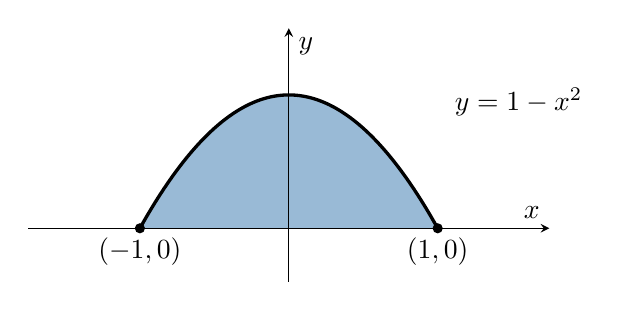
\begin{tikzpicture}
\begin{axis}[my style, axis on top, width=8.2cm, height=4.8cm,
  xmin=-1.75, xmax=1.75, ymin=-0.4, ymax=1.5,
  xtick=\empty, ytick=\empty, clip=false]
\addplot[draw=none, fill=solframe, fill opacity=0.55, domain=-1:1, samples=100] {1-x^2} \closedcycle;
\addplot[very thick, domain=-1:1, samples=100] {1-x^2};
\node[fill=black, circle, inner sep=1.3pt] at (axis cs:-1,0) {};
\node[fill=black, circle, inner sep=1.3pt] at (axis cs:1,0) {};
\node[below] at (axis cs:-1,0) {$(-1,0)$};
\node[below] at (axis cs:1,0) {$(1,0)$};
\node[anchor=west] at (axis cs:1.05,0.95) {$y=1-x^2$};
\end{axis}
\end{tikzpicture}
\end{center}
\begin{align*}
  m &\;=\; \rho\int_{-1}^{1}\left(1-x^2\right)dx \;=\; \rho\left[x-\frac{x^3}{3}\right]_{-1}^{1} \;=\; \frac{4\rho}{3},\\[6pt]
  M_x &\;=\; \rho\int_{-1}^{1}\frac{\left(1-x^2\right)^2}{2}\,dx
      \;=\; \frac{\rho}{2}\int_{-1}^{1}\left(1-2x^2+x^4\right)dx \\[6pt]
      &\;=\; \frac{\rho}{2}\left[x-\frac{2x^3}{3}+\frac{x^5}{5}\right]_{-1}^{1}
      \;=\; \frac{\rho}{2}\cdot\frac{16}{15} \;=\; \frac{8\rho}{15}.
\end{align*}
\[
\bar y=\frac{M_x}{m}=\frac{8\rho/15}{4\rho/3}=\frac{8}{15}\cdot\frac{3}{4}
\qquad
\boxed{\ \bar y=\frac{2}{5}\ }
\]
\end{solution}

  \item (BONUS 2 points) Find the $x$ coordinate of the centroid
    {\bf without using calculus}. Briefly justify your answer.

\begin{solution}
Replacing $x$ by $-x$ leaves both $y=1-x^2$ and $y=0$ unchanged, so the region is
symmetric about the $y$-axis and its centroid must lie on that axis.
\[
\boxed{\ \bar x=0\ }
\]
\end{solution}

  \end{enumerate}

\item (4 points) Compute the derivative of $f(x) = 5^{3x}$.

\begin{solution}
\[
f'(x)=5^{3x}\ln(5)\cdot\frac{d}{dx}(3x)
\]
\[
\boxed{\ f'(x)=3\ln(5)\,5^{3x}\ }
\]
\end{solution}

\end{enumerate}


\end{document}

%%% Local Variables:
%%% mode: latex
%%% TeX-master: t
%%% End:
